%-------------------------------------------------------------------------------
% 请勿删除本注释
% Free Response Question 3
%
% 指引:
% 如在小问之前有通用问题描述,请放置于此
%-------------------------------------------------------------------------------

\begin{figure}[H]
\centering
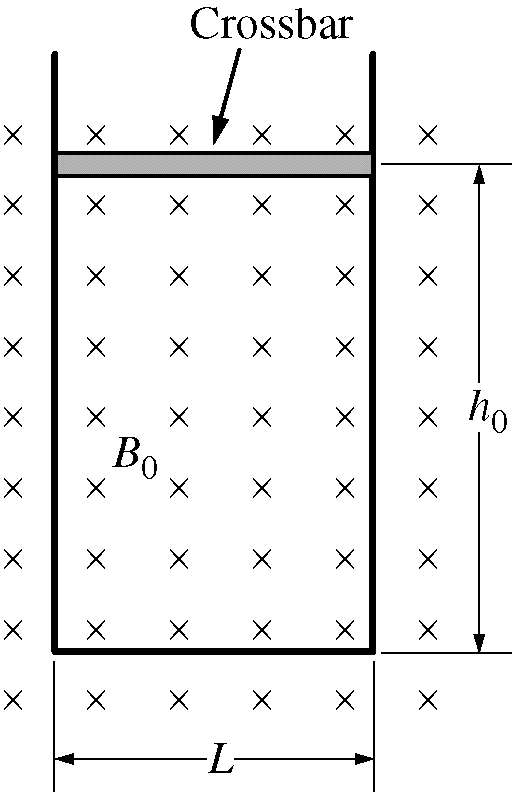
\includegraphics[scale=0.3]{images/img-018-033.png}
\end{figure}


\question
A closed loop is made of a U-shaped metal wire of negligible resistance and a movable metal crossbar of resistance $R$. The crossbar has mass $m$ and length $L$. It is initially located a distance $h_{0}$ from the other end of the loop. The loop is placed vertically in a uniform horizontal magnetic field of magnitude $B_{0}$ in the direction shown in the figure above. Express all algebraic answers to the questions below in terms of $B_{0}, L, m, h_{0}, R$, and fundamental constants, as appropriate. % 请删除并替换本行,与上一行 \question 之间不要留空行

\begin{parts}

%-------------------------------------------------------------------------------
% 请勿删除本注释
% Part (a)
%
% 指引:
% 如在小问之前有通用问题描述,请放置于此
%-------------------------------------------------------------------------------

\part
Determine the magnitude of the magnetic flux through the loop when the crossbar is in the position shown.  % 请删除并替换本行,与上一行 \part 之间不要留空行


The crossbar is released from rest and slides with negligible friction down the U-shaped wire without losing electrical contact.


%-------------------------------------------------------------------------------
% 请勿删除本注释
% Part (b)
%
% 指引:
% 如在小问之前有通用问题描述,请放置于此
%-------------------------------------------------------------------------------

\part
On the figure below, indicate the direction of the current in the crossbar as it falls. % 请删除并替换本行,与上一行 \part 之间不要留空行

\begin{figure}[h]
\centering

\includegraphics[scale=0.3]{images/img-018-034.png}
\end{figure}

Justify your answer.


%-------------------------------------------------------------------------------
% 请勿删除本注释
% Part (c)
%
% 指引:
% 如在小问之前有通用问题描述,请放置于此
%-------------------------------------------------------------------------------

\part
Calculate the magnitude of the current in the crossbar as it falls as a function of the crossbar's speed $v$. % 请删除并替换本行,与上一行 \part 之间不要留空行

%-------------------------------------------------------------------------------
% 请勿删除本注释
% Part (d)
%
% 指引:
% 如在小问之前有通用问题描述,请放置于此
%-------------------------------------------------------------------------------

\part
Derive, but do NOT solve, the differential equation that could be used to determine the speed $v$ of the crossbar as a function of time $t$. % 请删除并替换本行,与上一行 \part 之间不要留空行

%-------------------------------------------------------------------------------
% 请勿删除本注释
% Part (e)
%
% 指引:
% 如在小问之前有通用问题描述,请放置于此
%-------------------------------------------------------------------------------

\part
Determine the terminal speed $v_{T}$ of the crossbar. % 请删除并替换本行,与上一行 \part 之间不要留空行

%-------------------------------------------------------------------------------
% 请勿删除本注释
% Part (f)
%
% 指引:
% 如在小问之前有通用问题描述,请放置于此
%-------------------------------------------------------------------------------

\part
If the resistance $R$ of the crossbar is increased, does the terminal speed increase, decrease, or remain the same? % 请删除并替换本行,与上一行 \part 之间不要留空行

\underline{\qquad} Increases  \qquad    \underline{\qquad} Decreases  \qquad   \underline{\qquad} Remains the same

Give a physical justification for your answer in terms of the forces on the crossbar.

\end{parts}
